%===========================================================================
%	VI. Evaluation
%===========================================================================

\section{Kriterienbetrachtung}

Die zuvor definierten Vergleichskriterien finden nun Anwendung auf die entwickelten Apps. Die einzelnen Wertungen werden begründet, um zum Ende hin für die jeweilige App eine Kennzahl zu ermitteln, welche dann der Reflexion und der potenziellen Beantwortung der Forschungsfrage zugrunde liegen wird.

Es ist wichtig zu beachten, dass die exemplarische Entwicklung der nativen App innerhalb des iOS-Ökosystems nicht alleingestellt für die Gegenüberstellung zur \ac{pwa} verwendet werden kann. Bestimmte Aspekte können auf native Android-Entwicklung übertragen werden, andere werden wiederum außerhalb der Beispielanwendung begründet.

\subsection{Plattformabhängigkeit} \label{sec:6-plattform}
\input{main-matter/6_Evaluation/6-1_Plattformunabhaengigkeit.tex}


\subsection{Installation} \label{sec:6-installation}
\begin{tabbing}
	mmmmmmmmmmmmm				\= \kill
	\textbf{Wertung native App}: \> $++$ \\
	\textbf{Wertung \ac{pwa}}: \> \Circle
\end{tabbing}

\subsubsection{Bewertung native App}
Folgende Erkenntnisse basieren nicht auf der Entwicklung der Beispielanwendung, können jedoch zu einem ausreichenden Grad nachvollzogen werden (vgl. Abs. \ref{subsubsec:use-ios}), um sie in die Bewertung mit einfließen zu lassen.

 Native Anwendungen werden über einen zentralen Bezugspunkt gefunden, heruntergeladen und installiert. Der Nutzer kann über Stichpunkte und Suchbegriffe nach einer Vielzahl von Apps suchen und die gewünschte Anwendung herunterladen. Homepages, welche ihre Inhalte ebenfalls in Form von nativen Apps bereitstellen, zeigen dies oft in der Mobilversion ihrer Homepage an, sodass eine direkte Verknüpfung erstellt wird. Zwar könnte als Kritikpunkt angesehen werden, dass eine Homepage direkt als \ac{pwa} bezogen werden könnte. Dafür müsste jedoch jede Homepage die Möglichkeit einer \ac{pwa}-Installation bereitstellen, was zurzeit nicht der Fall ist.
 
 Sowohl unter dem Apple App Store als auch im Play Store von Google werden Apps vor ihrer Veröffentlichung geprüft, sodass keine Probleme (vor allem im Hinblick auf die Sicherheit des Endgerätes) bei der Benutzung entstehen. Es besteht in allen Fällen eine Qualitätskontrolle, welche unvorhersehbares Verhalten der bezogenen App vermeidet.
 
 Da sich kein unentkräftbares Argument gegen die Installationskriterien finden lässt, kann dieser Prozess mit gut bewertet werden.
 
\subsubsection{Bewertung \ac{pwa}}
Die \ac{pwa} wird über den Browser installiert. Daher ist die Installation stark abhängig vom verwendeten Browsertyp. Teilweise ist die Installation der Anwendung bedingt durch den Browser überhaupt nicht möglich. Bezogen auf den Desktopbrowser Chrome dürfte es in der Praxis häufig vorkommen, dass Nutzer die Bedienelemente zur Installation im Browser nicht als solche wahrnehmen (s. Abb. \ref{fig:dialog_install_pwa_desktop}). Dies wird als negativ gewertet.

Die Installation ist für den Nutzer nicht nachvollziehbar. Er sieht nicht, dass bzw. wie viele Daten bereits heruntergeladen wurden. Der ein oder andere Nutzer wird sich möglicherweise nicht bewusst sein, dass \textit{Zum Startbildschirm hinzufügen} eine tatsächliche Installation ausführt. Die Installation dauert je nach Komplexität der Webanwendung keine ganze bis wenige Sekunden. Die Deinstallation auf Android Geräten erfolgt wie bei nativen Apps. Bei der Desktop-\ac{pwa} ist diese unter Windows sogar deutlich einfacher, als bei Desktopanwendungen.

Insgesamt ist die Installation einer \ac{pwa} sehr einfach und mit nur einem Befehl des Nutzers ausführbar. Das gilt aber nur dann, wenn der Nutzer das Konzept der \ac{pwa} begriffen hat, was nach heutigem Stand wohl nicht der Fall sein dürfte. Die Installation selbst kommt ohne Lizenzvereinbarungen oder Installationspfade daher und ist außerdem bemerkenswert schnell.

Da einige störende Punkte für den Nutzer nicht optimal sind, die Installation insgesamt aber ein einfacher Prozess ist, erhält dieses Kriterium eine neutrale Wertung.

\subsection{Speicherzugriff} \label{sec:6-speicherzugriff}
\begin{tabbing}
	mmmmmmmmmmmmm				\= \kill
	\textbf{Wertung native App}: \> $++$\\
	\textbf{Wertung \ac{pwa}}: \> $+$
\end{tabbing}

\subsubsection{Bewertung native App}
Die Beispielanwendung nutzt die Bibliothek \texttt{CoreData}, welche es erlaubt, zu speichernde Dateistrukturen in Form von Datenbank-Design anzulegen und in den Benutzungsrahmen der App hinzuzufügen. Innerhalb der Android-Entwicklung existieren verschiedene Formen app-bezogenen Speichers, welche für unterschiedliche Zwecke verwendet werden können \cite{AndroidStorage}. In beiden Fällen bedarf es \textit{Endpoints}, welche das Verhalten des Speicherzyklus definieren.

Durch eine Speicherarchitektur, welche an relationale Datenbanken erinnert, können auch komplexe Speicherstrukturen entstehen, bspw. über die Definition verschiedener Speicherareale, welche in der Beispielanwendung keinen Nutzen fanden. Anders als bei \acp{pwa} existieren keine Einschränkungen von Dateiformaten.

Das Kriterium kann somit uneingeschränkt als gut bewertet werden, da zumindest in der Beispielanwendung keinerlei Grenzen des Speicherzugriffes aufgedeckt werden konnten.


\subsubsection{Bewertung \ac{pwa}}
Die \ac{pwa} hat keinen Zugriff auf das Dateisystem. Daten werden über den Browser im Speicher abgelegt, bspw. im Key-Value-Store \texttt{local storage}. Konfigurationen und Daten können auf diese Weise einfach gespeichert werden.

Das Speichern von binären Daten, wie  bpsw. Bildern, gestaltet sich in der Praxis schwierig. Es existieren uneinheitliche, browserspezifische Lösungen. Höchstwahrscheinlich kommt der Entwickler aber nicht um das Speichern binärer Daten als kodierten Text, z.B. \texttt{Base64}.

Das Kriterium wird als eher gut bewertet, weil mit dem Browserspeicher ein Großteil der Anwendungsfälle für Datenspeicherung abgedeckt ist und diese sehr einfach von Entwicklern genutzt werden können.

\subsection{Speicherbedarf} \label{sec:6-speicherbedarf}
\begin{tabbing}
	mmmmmmmmmmmmm				\= \kill
	\textbf{Wertung native App}: \> $+$\\
	\textbf{Wertung \ac{pwa}}: \> $++$
\end{tabbing}

\subsubsection{Bewertung native App}
Nach direkter Installation der Anwendung geben die Speicherinformationen der Systemeinstellungen des Testgerätes einen Bedarf von insgesamt 475 Kilobyte an. Pro To-Do-Eintrag wächst dieser um ca. 50 Kilobyte. Es lässt sich keine genaue Schätzung für eine äquivalente Android-App ableiten, weswegen dieser Gesichtspunkt wegfällt.

Da sich die native App auf Augenhöhe mit der \ac{pwa} befindet, jedoch einen hohen Bedarfszuwachs erfordert, wenn auf den Speicher der App geschrieben wird, wird dieses Kriterium mit eher gut bewertet.

\subsubsection{Bewertung \ac{pwa}}
Die implementierte Anwendung hat einen bemerkenswert kleinen Speicherbedarf von nur 356 Kilobyte. Der belegte Speicherplatz wächst unter Android nicht messbar (\textit{App-Info unter Einstellungen}) mit Anlegen neuer To-Do-Elemente. Daher wird dieses Kriterium uneingeschränkt mit gut bewertet.

\subsection{Aktualisierbarkeit} \label{sec:6-aktualisierbarkeit}
\textbf{Wertung native App}: $+$ \\ 
\textbf{Wertung \ac{pwa}}: $++$ 

\subsubsection{Bewertung native App}
Wie auch bei der Installation administriert der zentrale Bezugspunkt (Apple App Store resp. Google Play Store) auch die Aktualisierung der auf dem Gerät installierten Apps. Je nach Nutzereinstellungen werden diese automatisch bezogen oder der Nutzer wird benachrichtigt, dass Updates verfügbar sind.

Wie bereits erwähnt werden alle Aktualisierungen, welche vom Entwickler vertrieben werden, vor Veröffentlichung erneut geprüft. Dies stellt einen Vor- wie einen Nachteil dar. Grundsätzlich kann aufgrund des Qualitätsmanagements der Bezugspunkte von einer sicheren Distribution ausgegangen werden. Andererseits können relevante Hotfixes dadurch auch verzögert werden. Sollte der Nutzer die automatischen Updates deaktiviert haben, so kann es sein, dass dieser sicherheitsrelevante Aktualisierungen nicht mitbekommt oder bewusst ignoriert, was nicht im Sinne der Entwickler ist.

Verglichen mit \acp{pwa} kann der Nutzer alle Updates genau nachverfolgen, da parallel zu diesen auch Informationen über die neuen Inhalte, Bug-Fixes, etc. veröffentlicht werden können. Sollte eine Sicherheitslücke einer neuen Version bekannt werden, so kann der Nutzer diese ignorieren, bis eine weitere Version veröffentlicht wird, welche diese behebt.

Alles in allem gewinnen gewisse Pro- bzw. Contra-Argumente an Bedeutung, je nachdem, welche Position gerade betrachtet wird. Zusammengefasst kann die Aktualisierbarkeit aber mit eher gut bewertet werden, da der Prozess an sich funktioniert und für den Nutzer in jeder Hinsicht transparent ist, jedoch unter gewissen Umständen ignoriert werden kann.

\subsubsection{Bewertung \ac{pwa}}
Der Browser bzw. der laufende Service-Worker verwaltet das Caching und die Aktualisierung der Anwendung. Der Nutzer wird über Aktualisierungen nicht informiert. Er muss ihnen nicht zustimmen und kann sie nicht vermeiden. Entwickler müssen nur die neue Version der Anwendung deployen, damit die Installationen auf den Nutzergeräten aktualisiert werden.

Da vom Nutzer keine Aktion erforderlich ist und die Aktualisierung für Entwickler sehr einfach ist, erhält dieses Kriterium die eine gute Wertung.

\subsection{Design} \label{sec:6-konsistenz-des-designs}
\input{main-matter/6_Evaluation/6-6_Konsistenz_des_Designs}

\subsection{Bibliotheken} \label{sec:6-bibliotheken}
\textbf{Wertung native App}: $+$ \\
\textbf{Wertung \ac{pwa}}: $++$

\subsubsection{Bewertung native App}
Apple bietet für Swift eine Vielzahl von Bibliotheken an, eine Ergänzung bieten Drittanbieterbibliotheken, welche ebenfalls in die Entwicklungsumgebung eingebunden werden können. Bei letzterem ist \textit{CocoaPods} zu nennen (vgl. \cite{CocoaPods}). Gerade die direkte Unterstützung der eigenen Bibliotheken ermöglicht eine nahtlose Inklusion in den gesamten Entwicklungszyklus. Jedoch ist JavaScript wesentlich verbreiteter als Swift, weswegen das Volumen vorhandener Bibliotheken, welche die Entwicklung vereinfachen, deutlich größer ist. Die Android-Entwicklung ist jedoch ebenfalls sehr verbreitet, weswegen gerade dafür ebenfalls eine Vielzahl von Bibliotheken zur Verfügung steht.

Da die bloße Anzahl der insgesamt vorhandenen Bibliotheken der einzige Punkt ist, in welchem die native Entwicklung der Webentwicklung (und somit der \ac{pwa}-Entwicklung) nachsteht, kann das Kriterium mit eher gut bewertet werden.

\subsubsection{Bewertung \ac{pwa}}
Frameworks und Bibliotheken für JavaScript gibt es sprichwörtlich zu Tausenden. In der Praxis ist es ausgesprochen selten, zu einem Problem keine existierende (Teil-)Lösung in Form eines \texttt{npm}-Pakets zu finden. Die Nutzung und Installation dieser Pakete ist mit dem \texttt{npm}-Paketmanager einfach, automatisierbar und dürfte einen großen Teil zur Wahl der Programmiersprache JavaScript beitragen.

Dieses Kriterium ist eindeutig mit gut zu werten.

\subsection{Umsetzbarkeit} \label{sec:6-umsetzung}
\begin{tabbing}
	mmmmmmmmmmmmm				\= \kill
	\textbf{Wertung native App}: \> $++$ \\
	\textbf{Wertung \ac{pwa}}: \> $+$
\end{tabbing}

\subsubsection{Bewertung native App}
In puncto Umsetzbarkeit konnten alle Anforderungen der in Kapitel \ref{chap:architektur} definierten Architektur realisiert werden. Durch die durchgehende Nutzung der durch Apple empfohlenen Architekturstruktur \ac{mvc} war dies auch ohne größeren Aufwand oder die zwingende Nutzung von Umwegen möglich.

Im abgegrenzten Rahmen der Umsetzbarkeit wurden alle Anforderungen erfüllt, weswegen das Kriterium als gut bewertet werden kann.

\subsubsection{Bewertung \ac{pwa}}
Die Kombination aus dem Framework Angular, einer \ac{pwa} und der Hosting-Lösung Firebase funktioniert in der Praxis bemerkenswert reibungslos. Angular reduziert den Implementierungsaufwand gegenüber \textit{vanilla} JavaScript durch saubere Strukturierung der Anwendung in Komponenten und Services. In der Praxis war es nicht möglich, Benachrichtigungen ohne Netzwerkverbindung zu senden. Das ist ein großes Manko im Vergleich zur nativen App. Das Testen der \ac{pwa} war lokal nicht möglich bzw. mit nicht vertretbarem Aufwand realisierbar.

Dieses Kriterium ist mit eher gut zu werten.



\subsection{Testbarkeit} \label{sec:6-testbarkeit}
\input{main-matter/6_Evaluation/6-9_Testbarkeit}

\subsection{Vorausgesetzte Entwicklungserfahrung} \label{sec:6-vorausgesetzte-entwicklungserfahrung}
\textbf{Wertung native App}: $+$ \\
\textbf{Wertung \ac{pwa}}: $-$\\

\subsubsection{Bewertung native App}
Die Entwicklung einer iOS-App geschieht grundsätzlich innerhalb der Programmiersprache Swift. Diese greift jedoch auf Paradigmen des Vorgängers Objective-C zurück. Es werden zwar umfassende Kenntnisse \textit{nur} einer Programmiersprache benötigt, jedoch ist diese in ihrer Tragweite sehr umfangreich und folgt nicht immer den üblichen Entwicklungsmustern. Die Beispielanwendung lies sich ohne jegliche Drittanbieter-Bibliotheken umsetzen, weswegen die benötigten Dokumentationen der genutzten Funktionen überwiegend vom Betreiber Apple stammen, was zur Korrektheit und Aktualität dieser beiträgt. Positiv anzumerken ist ebenfalls die Tatsache, dass v.a. \ac{ui}-Konfigurationsschritte über den Interface Builder vereinfacht bzw. ersetzt werden können. Dies ist ebenfalls auf die Android-Entwicklung zu beziehen \cite{AndroidStudio}.

Da die Entwicklung in nativen Umgebungen durch verschiedene Lösungen vereinfacht wird und sich, verglichen mit \acp{pwa}, in \textit{einem} Umfeld aufhält, werden insgesamt weniger Voraussetzungen an den Entwickler gestellt. Auf der anderen Seite handelt es sich um sehr umfangreiche Programmierumgebungen, weswegen eine gewisse Erfahrung von Vorteil sein könnte. 

Insgesamt ist dieses Kriterium also mit eher gut zu bewerten.

\subsubsection{Bewertung \ac{pwa}}
Die \ac{pwa} setzt sich aus drei programmiersprachlichen Komponenten zusammen: JavaScript, \ac{html} und \ac{css}. Damit erfordert die Entwicklung sowohl Kenntnisse in prozeduraler Programmierung, als auch in der Implementierung passender \ac{html}- und \ac{css} Strukturen, welche letztendlich nur durch JavaScript modifiziert werden.

Außerdem ist zu erwähnen, dass komplexe JavaScript-Anwendungen ohne Frameworks und Bibliotheken in der Praxis selten zu finden sind. Die Nutzung von JavaScript ohne Angular, ReactJS, Vue.js, ö.Ä., ist mit nicht vertretbarem Aufwand verbunden. Da die Nutzung eines Frameworks quasi notwendig ist, aber es zwischen jenen deutliche Unterschiede gibt, zählt dies ganz klar zu den Wissensvoraussetzungen. Dazu kommen auch zwingend Kenntnisse der Linux-Kommandozeile für Node.js, \texttt{npm} und wahrscheinlich auch die eines \ac{cli}-Tools für das Deployment.

Die Wissenshürde ist deutlich erkennbar und für erfahrene Programmierer ohne Webkenntnisse dennoch vorhanden. Dieses Kriterium wird als negativ eingestuft.  

%\section{Nutzerfreundlichkeit} \label{sec:6-verstaendlichkeit}
%\textbf{Wertung \ac{pwa}}: neutral\\
\textbf{Wertung native App}:  \\



\subsection{\ac{pwa}}
Nutzer beziehen eine \ac{pwa} nicht über einen zentralen Markt, wie Apples App-Store, sondern über den Browser. Es ist davon auszugehen, dass Nutzer eine \ac{pwa} mehr aus Spontanität, als aufgrund gezielter Suche installieren. Es existiert, wie bereits erwähnt, kein Markt, auf welchem gezielt nach beispielsweise \texttt{Todo} gesucht werden kann. Es existieren nur einzelne Webanwendungen, die über eine Suchmaschine gefunden werden können. Vereinzelte Sammlungen von \ac{pwa}s existieren zwar, sind aber mit dem Bekanntheitsgrad des Apple oder Android App Markts nicht vergleichbar.

Es wird generell kein direkter Vor- oder Nachteil darin gesehen, dass ein Nutzer die \ac{pwa} von einer Webseite bezieht. Gegenüber einer nativen App, für welche eine Webseite auf einen externen App Markt verlinken muss ist dieser Prozess allerdings direkter und schneller.

Nicht zuletzt sollte erwähnt werden, dass für den Bezug einer \ac{pwa} kein Nutzerkonto benötigt wird.

Alles in Allem ist der Vertriebsweg für \ac{pwa}s noch sehr jung und gegenüber Apples AppStore tendenziell unausgereift. Allerdings besteht das Potenzial, dass Browserhersteller oder Suchmaschinen \ac{pwa}s mit in Suchergebnisse aufnehmen und so eine effektive Suche ermöglichen.

Dieses Kriterium befindet sich im neutralen Bereich. Da es jedoch die Möglichkeit der Installation von einer Webseite ohne einen Zwischenschritt gibt, wird dieses Kriterium als gut bewertet.

\section{Gesamtbetrachtung}
Für die Gesamtbetrachtung werden die Ergebnisse zur besseren Übersicht erneut in der Evaluationsmatrix (s. Tabelle \ref{tab:evaluationsmatrix_ausgefüllt}) dargestellt. Die Gesamtbewertung kann sich im Interval von 2,0 ($++$ oder gut) bis $-$2,0 ($--$ oder schlecht) befinden. 0,0 Verrechnungspunkte bilden die neutrale Mitte (\Circle).

 In der gewichteten Summe erhält die native App in der gewichteten Summe $1,1$ Verrechnungspunkte, was einer eher guten Wertung entspricht ($+$). Die \ac{pwa} liegt bei 0,55 Verrechnungspunkten. Das entspricht einer Wertung zwischen neutral (\Circle) und eher gut ($+$).
 
 \newpage

\begin{table}[t!]
	\centering
	\begin{tabular}{|l|c|c|c|}
		\hline
		\textbf{Kriterium}              & \textbf{Gesamtanteil} & \cellcolor{blue!25} \textbf{native App} & \cellcolor{green!25}\textbf{\ac{pwa}} \\
		
		\hline
		\multicolumn{4}{c}{\textbf{Anwendung}}         \\
		\hline
		\nameref{sec:6-plattform}   & 10\%         &\cellcolor{blue!25}$-$& \cellcolor{green!25}$+$ \\
		\nameref{sec:6-installation}           & 5\%           & \cellcolor{blue!25}$++$ & \cellcolor{green!25}\Circle \\
		\nameref{sec:6-speicherzugriff}        & 5\%          &\cellcolor{blue!25}$++$& \cellcolor{green!25}$+$ \\
		\nameref{sec:6-speicherbedarf}         & 5\%          &\cellcolor{blue!25}$+$&\cellcolor{green!25}$++$\\
		\nameref{sec:6-aktualisierbarkeit}     & 5\%          &\cellcolor{blue!25}$+$&\cellcolor{green!25}$++$ \\
		\nameref{sec:6-konsistenz-des-designs} & 5\%         &\cellcolor{blue!25}$+$& \cellcolor{green!25}$-$\\
		
		\hline
		\multicolumn{4}{c}{\textbf{Entwicklung}}      \\
		\hline
		\nameref{sec:6-bibliotheken}           & 10\%         &\cellcolor{blue!25}$+$&\cellcolor{green!25}$++$ \\
		\nameref{sec:6-umsetzung}              & 20\%         &\cellcolor{blue!25}$++$&\cellcolor{green!25}$+$ \\
		\nameref{sec:6-testbarkeit}            & 10\%         &\cellcolor{blue!25}\Circle &\cellcolor{green!25}$++$\\
		\nameref{sec:6-vorausgesetzte-entwicklungserfahrung}    & 10\%  &\cellcolor{blue!25}$+$&\cellcolor{green!25}$-$ \\
		\hline
		\hline
		\textbf{Gesamt}                  & \textbf{100\%}        &\cellcolor{blue!25}\textbf{1,1 ($+$)}& \cellcolor{green!25}\textbf{0,55 (\Circle/$+$)} \\
		\hline
	\end{tabular}
	\caption{Ergebnisse in der Evaluationsmatrix} \label{tab:evaluationsmatrix_ausgefüllt}
\end{table}
%	Plattformabhängikeit   & 0   & 1 & 2       & 3 & 4  & 10\%         \\
%Installation           & 0   & 1 & 2       & 3 & 4  & 5\%          \\
%Speicherzugriff        & 0   & 1 & 2       & 3 & 4  & 5\%          \\
%Speicherbedarf         & 0   & 1 & 2       & 3 & 4  & 5\%          \\
%Aktualisierbarkeit     & 0   & 1 & 2       & 3 & 4  & 5\%          \\
%Konsistenz des Designs & 0   & 1 & 2       & 3 & 4  & 5\%         \\
%Bibliotheken           & 0   & 1 & 2       & 3 & 4  & 10\%         \\
%Umsetzung              & 0   & 1 & 2       & 3 & 4  & 20\%         \\
%Testbarkeit            & 0   & 1 & 2       & 3 & 4  & 10\%         \\
%Vorausgesetzte Entwicklungserfahrung    & 0   & 1 & 2       & 3 & 4  & 10\%         \\
%Verständlichkeit       & 0   & 1 & 2       & 3 & 4  & 10\%         \\
%
\begin{figure}[h]

	\begin{tikzpicture}
	
		% Diagram setup
		\tkzKiviatDiagram[scale=1.0,label distance=.5cm,
		radial  = 4,
		gap     = 1,  
		lattice = 4]{
			Plattformabhängigkeit,
			Installation,
			Speicherzugriff,
			Speicherbedarf,
			Aktualisierbarkeit,
			Designs,
			Bibliotheken,
			Umsetzung,
			Testbarkeit,
			Vorausgesetzte Entwicklungserfahrung,
			Nutzerfreundlichkeit
		}
		
		% native App
		\tkzKiviatLine[thick,color=blue,mark=ball,
		fill=blue!20,opacity=.5](2,4,4,2,3,3,1,2,3,3,4)
		
		% PWA
		\tkzKiviatLine[thick,color=green,mark=ball,
		fill=green!20,opacity=.5](3,2,3,4,4,1,4,4,4,1,2)
		
		\tkzKiviatGrad[prefix=,unity=1,suffix=](0)  
	

	
	\end{tikzpicture}
	
	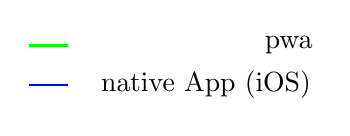
\begin{tikzpicture}
	%\draw[draw=black!20] (-0.1,-0.2) rectangle ++(15,0.5);
	
	\draw [thick, green] (0,0.5) -- (0.5,0.5); 
	\node at (3.3,0.5) {\acf{pwa}};
	
	\draw [thick, blue] (0,0) -- (0.5,0); 
	\node at (2.25,0) {native App (iOS)};
	

		\end{tikzpicture}
	
	\caption{Spinnennetzdiagram: Kriterienvergleich \acs{pwa} und native App}
\end{figure}

\newpage

Die einzelnen Kriterien werden im Netzdiagramm (s. Abb. \ref{fig:netzdiagramm}) visualisiert. Bei der Wertung ist zu beachten, dass die einzelnen Kriterien zwar gewichtet einfließen, jedoch gibt es unterschiedliche Interpretationsweisen für die einzelnen Kriterien. Diese Arbeit befindet sich dabei meist auf dem Standpunkt des Entwicklers und gewichtet die Anforderungen der Nutzer entsprechend geringer. Andere Forschungsansätze würden bei anderen Forschungsschwerpunkten zu abweichenden Interpretationen und Ergebnissen führen.

\section{Fazit}

Ob sich die \ac{pwa} etablieren kann, steht und fällt mit der zukünftigen Unterstützung durch Browserhersteller (insbesondere Apple Safari) aufgrund ihrer hohen Marktverbreitung. Es ist davon auszugehen, dass die Mehrheit der Nutzer ihren Browser nicht nach Kriterien der JavaScript-Unterstützung wählt und sie für die Nutzung von \acp{pwa} keinen neuen Browser herunterladen.

Es ist nach den Erkenntnissen dieser Arbeit jedoch fraglich, ob sich Apple grundsätzlich weiter mit \acp{pwa}beschäftigen wird. Das Konzept bietet für Entwickler großes Potenzial, da, verglichen mit nativer Implementierung, häufig eine doppelte Programmierung für Web und Apps entfällt. Aber gerade deshalb steht die \ac{pwa} in Konkurrenz zu Apples App Store. Mit der Entscheidung, \acp{pwa} zu unterstützen, gibt ein Hersteller die Kontrolle über die auf seinen Geräten installierten Apps ab. 
Möglicherweise würde man einen lukrativen Markt, nämlich den Verkauf von Software bzw. Apps, in die Hände einzelner Unternehmen geben.

Für Entwickler wäre dies jedenfalls erfreulich, da im Hinblick auf die schnelle Ausbreitung von JavaScript im Webbereich quasi für jedes Problem bereits eine Lösung existiert. Nicht zuletzt kommuniziert fast jede native App sowieso mit dem Internet, um dynamisch Daten zu laden und zu speichern. Ein Webentwickler könnte mit einer \ac{pwa} eine App entwickeln, ohne Spezialist für eine Plattform zu sein. Unter Verwendung von Node.js könnten App, Website und Webservices alle in der gleichen Sprache, nämlich JavaScript, entwickelt werden.

Bezieht man sich bei der Reflexion ausschließlich auf Anwendungen im Web, würden die meisten Webseiten von den Caching-Möglichkeiten der \ac{pwa} profitieren, Ladezeiten verkürzen können und dem Nutzer ein flüssigeres Gesamterlebnis bieten. Es ist davon auszugehen, dass sich das positiv auf die Kundeninteraktionen mit der Website auswirkt.
